\chapter{2. Random variable generation}
\section{Introduction}
\subsection{The inverse transformation}
\begin{center}
\begin{marginfigure}
  \centering
  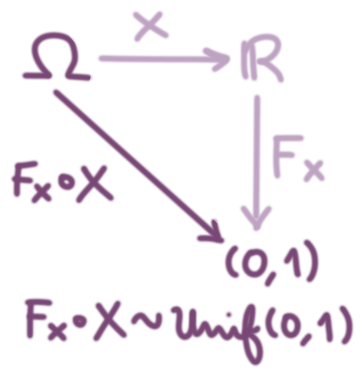
\includegraphics[scale=1]{26Feb_1.png}
\end{marginfigure}
\end{center}

\begin{teo}
\label{teo: inverse transf, teo 1}
(\textbf{p.44})
Sea $X$ una variable aletoria continua,
con funciones de densidad $f_{X}$ y $F_{X}$, respectivamente,
con $F_{X} : \IR \longrightarrow (0,1)$ invertible.
La variable aleatoria
\[
U=F_{X} \circ X
\]
tiene distribución $\mathcal{U}(0,1)$.
\end{teo}

\noindent
\textbf{Demostración.}
En efecto, sea $u \in (0,1)$. Puesto que por hipótesis
$F_{X}$ es invertible (o, equivalentemente,
biyectiva), existe un único $x \in \IR$ tal que
$F_{X}(x)=u$. Se tiene entonces que


\begin{align*}
P(U \leq u) = P (F_{X}(X) \leq F_{X}(x)) & =
P(F_{X}^{-1}(F_{X}(X)) \leq F_{X}^{-1}(F_{X}(X))) \\
= & P(X \leq x) = F_{X}(x)=u.
\end{align*}


\begin{figure}[H]
\centering
	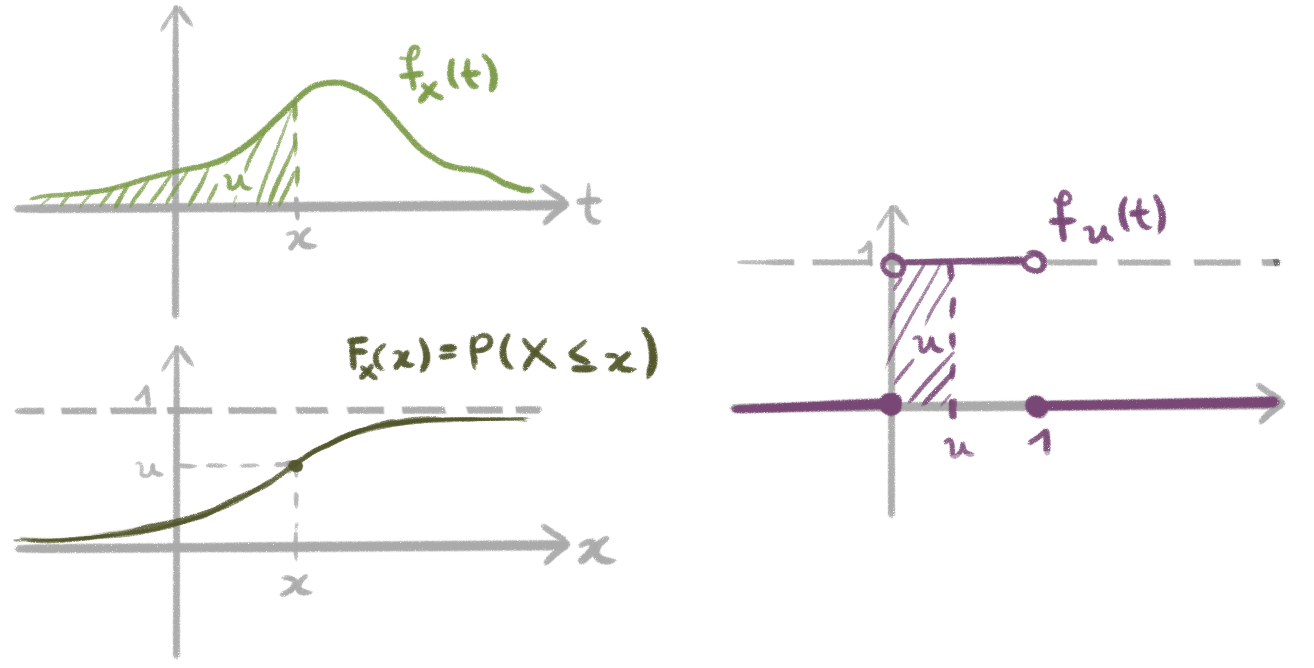
\includegraphics[scale=0.8]{26Feb_2} 
	\caption{a}
\end{figure}

\QEDB
\vspace{0.2cm}







El resultado dual se da a continuación.

\begin{center}
\begin{marginfigure}
  \centering
  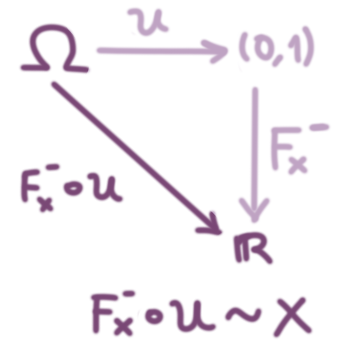
\includegraphics[scale=1]{26Feb_3.png}
\end{marginfigure}
\end{center}
\begin{ejercicio}
\label{ejerc: 2.1}
(\textbf{2.1, p.44})
Si $X$ es una variable aleatoria con función de
acumulación $F_{X}$, defina a la \textbf{inversa generalizada
de $F_{X}$} como sigue:

\begin{equation}
\forall u \in (0,1): \hspace*{0.2cm}
F_{X}^{-}(u):= inf\{x \hspace{0.1cm} : \hspace*{0.1cm} F_{X}(x) \geq u \}.
\end{equation}

Demuestre que si $U$ es una variable aleatoria con
distribución $U(0,1)$, entonces 
\[
F_{X}^{-} \circ U \sim X.
\]
\end{ejercicio}
\noindent
\textbf{Demostración.}

\begin{center}
\begin{marginfigure}
  \centering
  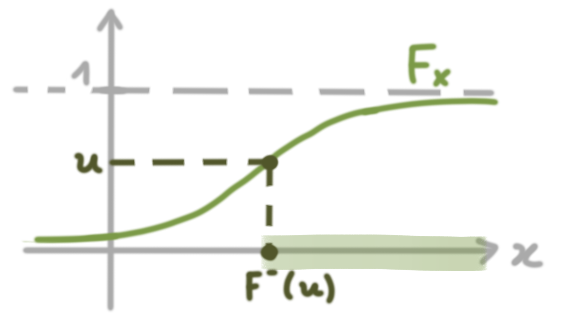
\includegraphics[scale=1]{26Feb_4.png}
  \caption{Definición de $F^{-}_{X}$.}
\end{marginfigure}
\end{center}


Sea $Y: \Om \longrightarrow \IR$ la composición
$F^{-}_{X} \circ U$. Debemos demostrar que

\begin{equation*}
\forall z \in \IR: \hspace*{0.2cm}
P(Y \leq z) = P(X \leq z).
\end{equation*}


Sea pues $z \in \IR$.

\begin{itemize}
\item[a)] Por ser $F_{X}$ una función de acumulación, es 
una función creciente, luego, los eventos
\[
(X \leq z) \hspace{0.2cm} \text{y} \hspace{0.2cm} 
(F_{X}(X) \leq F_{X}(z))
\]

son iguales; además, según el teorema 
\ref{teo: inverse transf, teo 1}, $F \circ X \sim U$; así,
\begin{equation}
\label{eq0: 26Feb}
P(X \leq z) = P(F_{X}(X) \leq F_{X}(z)) = P(U \leq F_{X}(z)).
\end{equation}

\item[b)] Por la definición de $F^{-}$ en términos de un 
ínfimo, se sigue de inmediato que
\begin{align*}
P(Y \leq z) = P(F^{-}_{X}(U) \leq z) = & 
P (\{w \in \Omega \hspace{0.1cm} : \hspace{0.1cm} F^{-}_{X}(U(w)) \leq z \}) \\
= & 
P (\{w \in \Omega \hspace{0.1cm} : \hspace{0.1cm} U(w) \leq F_{X}(z) \})
=P(U \leq F_{X}(z)),
\end{align*}

o sea, que 
\begin{equation}
\label{eq1: 26Feb}
P(Y \leq z) = P(U \leq F_{X}(z));
\end{equation}
\end{itemize}

de \eqref{eq0: 26Feb} y \eqref{eq1: 26Feb} se sigue,
como queríamos, que
$P(X \leq z) = P(Y \leq z)$.

\QEDB
\vspace{0.2cm}



\begin{ejercicio}
(\textbf{2.2, p. 45}) Se dan algunas funciones de probabilidad.
Calcule las correspondientes funciones de acumulación, y en base a
estas y los resultados anteriores, simule via una transformación
de variables aleatorias uniformes la distribución dada.
Comparar el resultado obtenido con las gráficas hechas
llamando a la distribución en R.
\end{ejercicio}

\noindent
\textbf{Solución}

\begin{itemize}
\item[a)] \textbf{Distribución logística}: la pdf es
\begin{equation}
\label{eq2: 26Feb}
f(x)= \frac{1}{\beta} \frac{e^{-(x- \mu)/ \beta}}{(1+e^{-(x- \mu)/ \beta})^{2}}
\end{equation}
(al parámetro $\mu$ se le llama \textbf{localización}, y al $\beta$
\textbf{escala}). Integrando, calculamos que

\[
\forall x \in \IR : \hspace{0.2cm}
F(x)= \frac{1}{1+e^{-(x-\mu)/\beta}};
\]
la inversa de esta función es 

\[
F^{-1}(u)= ln \left( \left( \frac{u}{1-u}  \right)^{\beta} \right) + \mu,
\]
luego, según el ejercicio \ref{ejerc: 2.1}, si $U \sim U(0,1)$, la variable
aleatoria
\[
Y = ln \left( \left( \frac{U}{1-U}  \right)^{\beta} \right) + \mu
\]
tiene a la función \eqref{eq2: 26Feb} como función de distribución.

Los valores de default de los parámetros de la distribución logística
en \texttt{rstudio} son 
\[
\mu=0, \hspace{0.2cm} \beta=1;
\]
a continuación comprobamos con un experimento numérico
en \texttt{rstudio} que las variables aleatorias
\begin{equation}
\label{eq3: 26Feb}
X = logistic(\mu=0, \beta=1) \hspace{0.2cm} \text{y}
\hspace{0.2cm} Y= ln \left( \frac{U}{1-U} \right)
\end{equation}
parecen tener la misma distribución.
\end{itemize}

\begin{figure}[H]
\centering
	\sidecaption{Histogramas de distribuciones logísticas
	(tamaño de muestra: $10^{4}$) usando las variables aleatorias
	\eqref{eq3: 26Feb}.}
	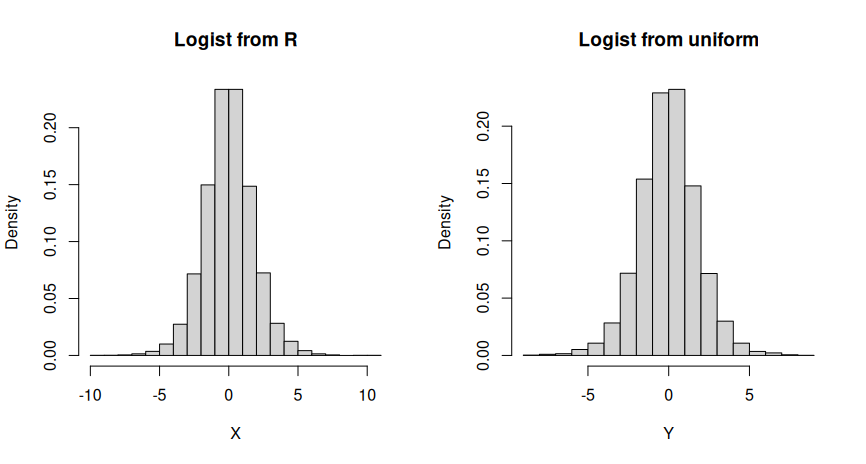
\includegraphics[scale=0.5]{logistic} 
\end{figure}
Código de R empleado para generar la imagen:
\begin{verbatim}
> Nsim=10^4
> U=runif(Nsim)
> X=rlogis(Nsim)
> Y=log(U/(1-U))
> par(mfrow=c(1,2))
> hist(X, freq=FALSE, main='Logist from R')
> hist(Y, freq=FALSE, main='Logist from uniform')
\end{verbatim}


\vspace{0.2cm}






